\documentclass[10pt,a4paper,landscape]{article}
\usepackage[margin=12mm]{geometry}
\usepackage{graphicx,amsmath}
\usepackage[T1]{fontenc}
\usepackage{newtxtext,newtxmath}
\usepackage[font=small,labelfont=bf]{caption}
\pagestyle{empty}
\setlength{\parindent}{0pt}
\begin{document}
{\large\bfseries Figure 3 comparison with five-cycle MPC}\hfill Original article initial condition, $1\times$\par
\begin{figure}[h!]
\centering
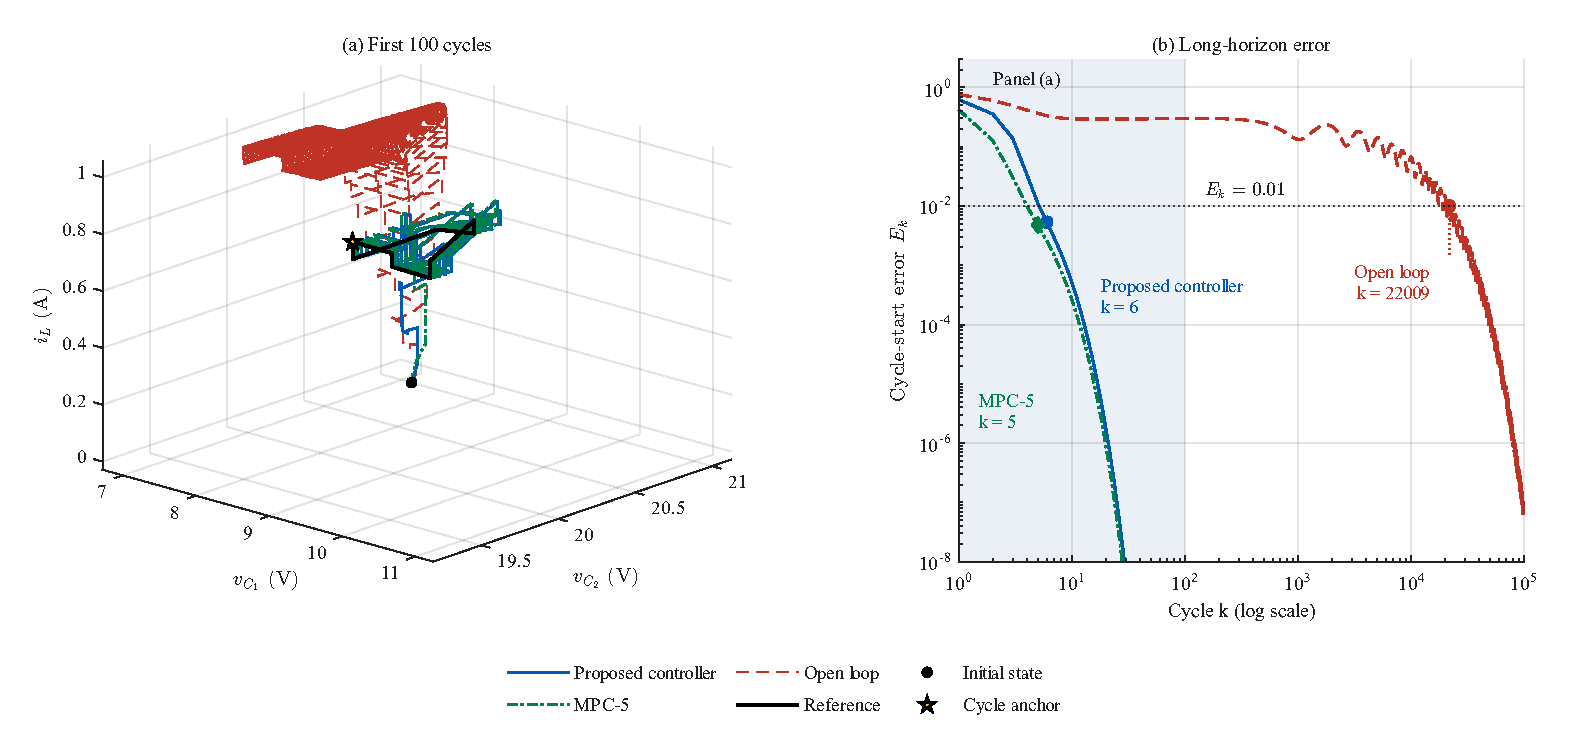
\includegraphics[width=26.6cm]{trajectory-comparison.pdf}
\setcounter{figure}{2}
\caption{Exact switched-affine responses with the proposed controller, MPC-5, the nominal open loop, and the periodic reference. Panel (a) retains 30 exact samples per mode interval over 100 cycles for each response, with each controller's own switching instants. Panel (b) uses actual cycle-start samples: both controllers stop at $k=100$, while the saved open-loop record extends to $k=100000$. The shaded range identifies panel (a). Markers show the first samples below $E_k=0.01$ for the proposed controller, $k=6$, and MPC-5, $k=5$, and the persistent crossing for open loop, $k=22009$, after which all saved samples remain below the threshold. No controller extrapolation or error flooring is used; values below $10^{-8}$ lie outside the displayed range.}
\end{figure}
\vspace{-2mm}
\noindent\textbf{Simulation conditions.}
The article plant and reconciled nine-interval schedule use $T=286\,\mu\mathrm{s}$ and applied dwell bound $3\,\mu\mathrm{s}$.
The initial state is $x_0=(7.5143,\;20.8211,\;0.0314)^\top$ in V, V, A;
the cycle anchor is $\bar{x}(0)=(9.9247,\;19.2928,\;0.9823)^\top$.
The error is $E_k=\|S_x^{-1}(x_k-\bar{x}(0))\|_2$, with $S_x=\operatorname{diag}(10,20,1)$ and timing scale $10\,\mu\mathrm{s}$.
Both controllers use relative weights $Q=I$, $R=0.001I$.
MPC-5 retains the native invariant terminal set and terminal LQR cost, with the equivalent cost scaling $Q=1000I$, $R=I$.
All 100 QPs succeeded. Dwell, period, exact dense endpoints, normalization, and agreement with the saved $1\times$ study passed local checks. This comparison is simulation evidence, not a global nonlinear stability or embedded timing guarantee.
\end{document}
